\documentclass[14pt]{beamer}
\usepackage{./Estilos/BeamerUVM}
\usepackage{./Estilos/ColoresLatex}
%Sección para el tema de beamer, con el theme, usercolortheme y sección de footers
\usetheme{CambridgeUS}
\usecolortheme{wolverine}
%\useoutertheme{default}
\setbeamercovered{invisible}
% or whatever (possibly just delete it)
\setbeamertemplate{section in toc}[sections numbered]
\setbeamertemplate{subsection in toc}[subsections numbered]
\setbeamertemplate{subsection in toc}{\leavevmode\leftskip=3.2em\rlap{\hskip-2em\inserttocsectionnumber.\inserttocsubsectionnumber}\inserttocsubsection\par}
%\setbeamercolor{section in toc}{fg=blue}
%\setbeamercolor{subsection in toc}{fg=blue}
%\setbeamercolor{frametitle}{fg=blue}
\setbeamertemplate{caption}[numbered]

\setbeamertemplate{footline}
\beamertemplatenavigationsymbolsempty
\setbeamertemplate{headline}{}


\makeatletter
\setbeamercolor{secºtion in foot}{bg=gray!30, fg=black!90!orange}
\setbeamercolor{subsection in foot}{bg=blue!30!yellow, fg=red}
\setbeamercolor{date in foot}{bg=black, fg=white}
\setbeamertemplate{footline}
{
  \leavevmode%
  \hbox{%
  \begin{beamercolorbox}[wd=.333333\paperwidth,ht=2.25ex,dp=1ex,center]{section in foot}%
    \usebeamerfont{section in foot} \insertsection
  \end{beamercolorbox}%
  \begin{beamercolorbox}[wd=.333333\paperwidth,ht=2.25ex,dp=1ex,center]{subsection in foot}%
    \usebeamerfont{subsection in foot}  \insertsubsection
  \end{beamercolorbox}%
  \begin{beamercolorbox}[wd=.333333\paperwidth,ht=2.25ex,dp=1ex,right]{date in head/foot}%
    \usebeamerfont{date in head/foot} \insertshortdate{} \hspace*{2em}
    \insertframenumber{} / \inserttotalframenumber \hspace*{2ex} 
  \end{beamercolorbox}}%
  \vskip0pt%
}






% \usefonttheme{serif}
\usepackage[clock]{ifsym}
\DeclareSIUnit\erg{erg}
\DeclareSIUnit[number-unit-product = {\,}]\cal{cal}

\sisetup{per-mode=symbol}
\resetcounteronoverlays{saveenumi}

% Macro para agregar el logo de UVM en cada slide de la presentación

\addtobeamertemplate{frametitle}{}{%
\begin{tikzpicture}[remember picture,overlay]
\coordinate (logo) at ([xshift=-1.5cm,yshift=-0.8cm]current page.north east);
% \fill[devryblue] (logo) circle (.9cm);
% \clip (logo) circle (.75cm);
\node at (logo) {
\includegraphics[width=2.1cm]{Imagenes/logo_UVM.png}};
\end{tikzpicture}}


\title{\Large{Electricidad} \\ \normalsize{Física IV (Área II)}}
\date{}

\begin{document}
\maketitle

\section*{Contenido}
\frame[allowframebreaks]{\frametitle{Contenido} \tableofcontents[currentsection, hideallsubsections]}

\section{Electricidad}
\frame[allowframebreaks]{\tableofcontents[currentsection, hideothersubsections]}
\subsection{Introducción}

\begin{frame}
\frametitle{¿Qué es la electricidad?}
La electricidad se define como un fenómeno físico que se origina del \textocolor{flame}{movimiento de cargas eléctricas} a través de la atracción y repulsión de las mismas.
\end{frame}
\begin{frame}
\frametitle{¿Qué es la electricidad?}
La electricidad es una rama de la Física que estudia todos los \textocolor{ao}{fenómenos relacionados con las cargas eléctricas} en reposo o movimiento.
\end{frame}
\begin{frame}
\frametitle{Electrostática}
Es la rama de la electricidad que se encarga de estudiar las \textocolor{folly}{cargas eléctricas en reposo}.
\end{frame}
\begin{frame}
\frametitle{Electrodinámica}
Es la rama de la electricidad que se encarga de estudiar las \textocolor{halayaube}{cargas eléctricas en movimiento}.
\end{frame}
\begin{frame}
\frametitle{Tipos de carga eléctrica}
Las cargas eléctricas son de dos tipos:
\pause
\begin{figure}
    \centering
    \begin{tikzpicture}
        \node at (0, 0) {Tipos de carga};
        \draw node at (4.75, 1) {Carga positiva};
        \draw [-stealth] (2, 0) -- (3, 1);
        \draw [fill, color=ao, text=white] (7.5, 1) circle (10pt) node {$+$};

        \draw node at (4.75, -1) {Carga negativa};
        \draw [-stealth] (2, 0) -- (3, -1);
        \draw [fill, color=red, text=white] (7.5, -1) circle (10pt) node {$-$};
        
    \end{tikzpicture}
\end{figure}
\end{frame}
\begin{frame}
\frametitle{La carga eléctrica}
Se denomina \textocolor{ballblue}{carga eléctrica elemental} y se denota como:
\pause
\begin{itemize}
\item Carga positiva $+e$, $e^{+}$
\item Carga negativa $-e$, $e^{-}$
\end{itemize}
\end{frame}
\begin{frame}
\frametitle{El valor de $e$}
El valor de la carga eléctrica $e$ es:
\pause
\begin{align*}
e = \SI{1.6d-19}{\coulomb}
\end{align*}
\pause
Entonces:
\begin{itemize}
\item Carga positiva $+e, \, e^{+} = + \SI{1.6d-19}{\coulomb}$
\item Carga negativa $-e, \, e^{-} = -\SI{1.6d-19}{\coulomb}$
\end{itemize}    
\end{frame}
\begin{frame}
\frametitle{Interacción entre cargas eléctricas}
La relación entre cargas eléctricas con signo, se presenta a continuación:
\end{frame}
\begin{frame}
\frametitle{Ley de atracción}
\textocolor{airforceblue}{Cargas con signo contrario se atraen}.
\begin{figure}
    \centering
    \begin{tikzpicture}
        \draw [fill, color=ao, text=white] (0, 0) circle (10pt) node {$+$};
        \draw[-{Triangle[width=18pt,length=8pt]}, line width=10pt](1, 0) -- (2, 0);
        \draw[-{Triangle[width=18pt,length=8pt]}, line width=10pt](4, 0) -- (3, 0);
        \draw [fill, color=red, text=white] (5, 0) circle (10pt) node {$-$};
    \end{tikzpicture}
\end{figure}
\end{frame}
\begin{frame}
\frametitle{Ley de repulsión}
\textocolor{ao(english)}{Cargas con signo igual se repelen}.
\begin{figure}
    \centering
    \begin{tikzpicture}
        \draw [fill, color=ao, text=white] (0, 0) circle (10pt) node {$+$};
        \draw[-{Triangle[width=18pt,length=8pt]}, line width=10pt](-0.5, 0) -- (-1.5, 0);
        \draw[-{Triangle[width=18pt,length=8pt]}, line width=10pt](3, 0) -- (4, 0);
        \draw [fill, color=ao, text=white] (2.5, 0) circle (10pt) node {$+$};

        \draw [fill, color=red, text=white] (0, -1.5) circle (10pt) node {$-$};
        \draw[-{Triangle[width=18pt,length=8pt]}, line width=10pt](-0.5, -1.5) -- (-1.5, -1.5);
        \draw[-{Triangle[width=18pt,length=8pt]}, line width=10pt](3, -1.5) -- (4, -1.5);
        \draw [fill, color=red, text=white] (2.5, -1.5) circle (10pt) node {$-$};
        
    \end{tikzpicture}
\end{figure}
\end{frame}
\begin{frame}
\frametitle{Una ley importante}
\textocolor{ceruleanblue}{Conservación de la carga eléctrica}.
\\
\bigskip
La carga eléctrica no se crea ni se destruye, solo se transforma de un cuerpo o material a otro.
\end{frame}

\section{Tipos de materiales}
\frame[allowframebreaks]{\tableofcontents[currentsection, hideothersubsections]}
\subsection{Conductor}

\begin{frame}
\frametitle{El material conductor}
Un medio o material que \textocolor{burgundy}{permite el movimiento} de las cargas eléctricas (electrones)
en respuesta a una fuerza eléctrica, se denomina \textocolor{cobalt}{conductor}.
\end{frame}
\begin{frame}
\frametitle{El material conductor}    
Los materiales conductores son los que se pueden electrizar en toda su superficie, debido a que los electrones se mueven libremente.
\\
\bigskip
\pause
Los metales por lo general son buenos conductores de la electricidad.
\end{frame}
\begin{frame}
\frametitle{Materiales conductores}
\begin{figure}
    \centering
    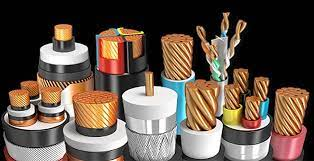
\includegraphics[scale=0.8]{Imagenes/Materiales_Conductores_01.jpg}
\end{figure}
\end{frame}
\begin{frame}
\frametitle{Materiales resistivos}
\begin{figure}
    \centering
    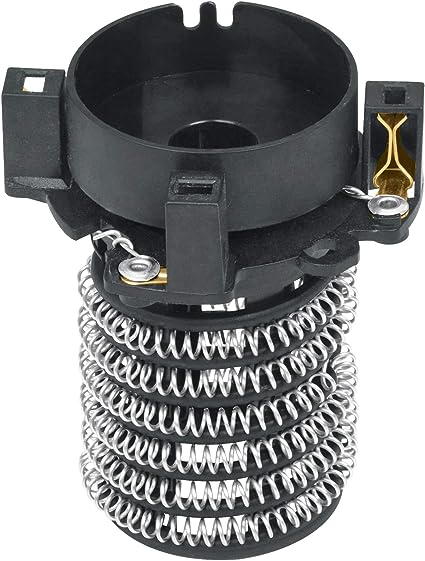
\includegraphics[scale=0.3]{Imagenes/Materiales_Conductores_02.jpg}
\end{figure}
\end{frame}
\begin{frame}
\frametitle{La resistividad eléctrica}
La resistividad de un material es una medida de la fuerza con la que un material se opone al flujo de la corriente eléctrica.
\end{frame}
\begin{frame}
\frametitle{La resistividad eléctrica}
El símbolo de la resistividad es la letra griega minúscula rho,
\end{frame}
\begin{frame}
\frametitle{Conductores}
\vspace*{-1cm}
\begin{table}
\setlength{\tabcolsep}{1pt}
\centering
\begin{tabular}{c | c}
Material & Resistividad (\si{\ohm\meter}) \\ \hline
Plata & \num{1.59d-8} \\ \hline
Cobre & \num{1.68d-8} \\ \hline
Oro & \num{2.44d-8} \\ \hline
Aluminio & \num{2.65d-8} \\ \hline
\end{tabular}
\end{table}
\end{frame}
    
\subsection{Aislantes}

\begin{frame}
\frametitle{Los aislantes}
Los materiales que no permiten que las partículas cargadas se muevan hacia otra región del material debido a una fuerza eléctrica, son llamados \textocolor{coolblack}{aislantes} por ejemplo, la madera.
\end{frame}
\begin{frame}
\frametitle{Aislantes}
\begin{table}
\vspace*{-1cm}
\centering
\begin{tabular}{c | c}
Material & Resistividad (\si{\ohm\meter}) \\ \hline
Ámbar & \num{5d14} \\ \hline
Vidrio & \num{d9} - \num{d14} \\ \hline
Mica & \num{d11} - \num{d15} \\ \hline
Azufre & \num{d15} \\ \hline
\end{tabular}
\end{table}
\end{frame}

\subsection{Semiconductores}

\begin{frame}
\frametitle{Los materiales semiconductores}
Existen otros tipos de materiales cuyas propiedades son intermedias entre los conductores y aislantes: \pause  se llaman \textocolor{cornellred}{semiconductores}.
\end{frame}
\begin{frame}
\frametitle{Base de la electrónica}
Los materiales semiconductores con mayor utilidad en la electrónica son el silicio y el germanio.
\end{frame}
\begin{frame}
\frametitle{Semiconductores}
\begin{table}
\centering
\begin{tabular}{c | c}
Material & Resistividad (\si{\ohm\meter}) \\ \hline
Carbono & \num{3.5d-5} \\ \hline
Germanio & \num{600d-3} \\ \hline
Silicio & \num{2.300} \\ \hline
\end{tabular}
\end{table}
\end{frame}

\section{Ley de Ohm}
\frame{\tableofcontents[currentsection, hideothersubsections]}
\subsection{La corriente}

\begin{frame}
\frametitle{La corriente eléctrica}
El flujo de las partículas cargadas es lo que se conoce como \textocolor{red}{corriente eléctrica}.
\end{frame}
\begin{frame}
\frametitle{La unidad de corriente}
La unidad de corriente eléctrica es el \textocolor{ao}{Ampere}, su símbolo es \si{\ampere}
\end{frame}
\begin{frame}
\frametitle{La corriente eléctrica}
Las partículas cargadas en una cierta dirección de un conductor chocan con los átomos, \pause produciendo una pérdida de energía que se manifiesta en forma de calor.
\end{frame}

\subsection{El voltaje}

\begin{frame}
\frametitle{El voltaje}
El \textocolor{cobalt}{voltaje}, \pause también conocido como \textocolor{amethyst}{diferencia de potencial eléctrico}.
\end{frame}
\begin{frame}
\frametitle{El voltaje}
El voltaje se puede ver como la \textocolor{cadmiumgreen}{fuerza impulsora} que permite que la corriente eléctrica fluya a través de los conductores.
\end{frame}
\begin{frame}
\frametitle{El voltaje}
Sus unidades son los \textocolor{brown(web)}{voltios} y su símbolo es \si{\volt}
\end{frame}

\subsection{La resistencia}

\begin{frame}
\frametitle{La resistencia eléctrica}
Una medida de \textocolor{blue}{oposición} que presentan las partículas cargadas al moverse libremente en una cierta dirección de un material conductor \pause es lo que se conoce como \textocolor{cerise}{resistencia eléctrica}.
\end{frame}
\begin{frame}
\frametitle{Unidades de la resistencia}
La unidad de la resistencia eléctrica es el \textocolor{carnelian}{Ohm}.
\\
\bigskip
\pause
Su símbolo es $\Omega$
\end{frame}

\subsection{Relación entre las variables}

\begin{frame}
\frametitle{La ley de Ohm}
La \textocolor{cornellred}{ley de Ohm} fue formulada por el físico alemán George Simon Ohm.
\end{frame}
\begin{frame}
\frametitle{La ley de Ohm}
En un circuito eléctrico describe la relación entre:
\pause
\setbeamercolor{item projected}{bg=corn,fg=black}
\setbeamertemplate{enumerate items}{%
\usebeamercolor[bg]{item projected}%
\raisebox{1.5pt}{\colorbox{bg}{\color{fg}\footnotesize\insertenumlabel}}%
}
\begin{enumerate}[<+->]
\item La corriente eléctrica $(I)$
\item La diferencia de potencial o voltaje $(V)$
\item La resistencia eléctrica $(R)$
\end{enumerate}
\end{frame}
\begin{frame}
\frametitle{La ley de Ohm}
La ley de Ohm se expresa matemáticamente mediante la siguiente ecuación:
\pause
\begin{align*}
V = I \, R
\end{align*}
\end{frame}
\begin{frame}
\frametitle{Ejercicios}
\setbeamercolor{item projected}{bg=denim,fg=white}
\setbeamertemplate{enumerate items}{%
\usebeamercolor[bg]{item projected}%
\raisebox{1.5pt}{\colorbox{bg}{\color{fg}\footnotesize\insertenumlabel}}%
}
\begin{enumerate}[<+->]
\item Un tostador eléctrico tiene una resistencia de \SI{30}{\ohm} cuando está caliente. ¿Cuál será la intensidad de la corriente que fluirá al conectarlo a una línea de \SI{120}{\volt}?
\seti
\end{enumerate}
\end{frame}
\begin{frame}
\frametitle{Ejercicios}
\setbeamercolor{item projected}{bg=denim,fg=white}
\setbeamertemplate{enumerate items}{%
\usebeamercolor[bg]{item projected}%
\raisebox{1.5pt}{\colorbox{bg}{\color{fg}\footnotesize\insertenumlabel}}%
}
\begin{enumerate}[<+->]
\conti
\item Determina la intensidad de la corriente eléctrica a través de una resistencia de \SI{50}{\ohm} al aplicarle una diferencia de potencial de \SI{120}{\volt}.
\seti
\end{enumerate}
\end{frame}
\begin{frame}
\frametitle{Ejercicios}
\setbeamercolor{item projected}{bg=denim,fg=white}
\setbeamertemplate{enumerate items}{%
\usebeamercolor[bg]{item projected}%
\raisebox{1.5pt}{\colorbox{bg}{\color{fg}\footnotesize\insertenumlabel}}%
}
\begin{enumerate}[<+->]
\conti
\item Un alambre conductor deja pasar \SI{7}{\ampere} al aplicarle una diferencia de potencial de \SI{110}{\volt}. ¿Cuál es su resistencia?
\end{enumerate}
\end{frame}
    
\end{document}